%\documentclass[../main.tex]{subfiles}
%\begin{document}
\emph{Process mining} is a relatively new discipline that bridges the gap of data mining and business process management. The objective of process mining is to support the analysis of business processes, provide valuable insights in processes and further improve the business execution based on the business execution data which are recorded in event logs. According to  \cite{van2011process}, process mining techniques are divided into three categories: \emph{process discovery}, \emph{conformance checking}, and \emph{process enhancement}. \emph{Process discovery} techniques derive visual models from event logs of information systems, aiming at a better understanding of real business processes. \emph{Conformance checking} analyzes the deviations between a reference process model and observed behaviors driven from its execution. \emph{Process enhancement} adapts and improves existing process models by extending the models with additional data perspectives or repairing the reference models to accurately reflect observed behaviors. 

Most of the organizations have predefined process execution rules of activities which are captured in a process model. One execution of related activities in this model is called a trace. A trace which has no deviation to the model is a fitting trace. However, in practice, business processes often encounter exceptional situations where it is necessary to execute process differing from the reference model. With accumulation of deviations, the reference process model needs amending to reflect reality. 


Basically, one can apply process discovery techniques again on the event log to obtain a new model. This method is referred as process rediscovery.  Without consideration of the reference models, the rediscovered models are likely to differ a lot from the reference ones. However, there is a need that the improved model should be as similar as possible to the original model while replaying the current process execution \cite{fahland2012repairing}. In this situation, the rediscovery method tends to fail due to the ignorance of the impact from the existing model. To meet this need, \textbf{model repair} techniques are proposed in  \cite{fahland2012repairing}.

\emph{Model repair} belongs to process enhancement \cite{fahland2012repairing}. It analyzes the workflow deviations between an event log and a process model, and fixes the deviations mainly by adding subprocesses on the model. As known, organizations are goal-oriented and aim to have high performance according to a set of Key Performance Indicator(KPI)s, e.g., the production time for a car industry, the logistic cost for importer companies.  However, little research in process mining is conducted on the basis of business performance \cite{ghasemi2019event}.  The authors of  \cite{ghasemi2019event} point out several contributions e.g.,   \cite{dees2017enhancing} to consider business performance into process mining. The work in  \cite{dees2017enhancing} divides deviations of model and the event log into positive and negative according to certain KPIs. Then it applies repair techniques in  \cite{fahland2012repairing} only with positive deviations which are deviations leading to positive KPI outcomes. This reason behind this approach  is to avoid introducing negative instances into the repaired model. 

However, the current repair methods have limits. Model repair techniques fix the model by adding subprocesses. They guarantee that the repaired model replays the whole event log but overgeneralizes the model, such that more behaviors are allowed than expected. Furthermore, the model complexity increases due to the repair techniques in \cite{fahland2012repairing}.  The work in \cite{dees2017enhancing} takes the performance into account but only uses deviations with positive performance outcomes to repair the model. Without consideration negative information, it is difficult for the repaired model to block the behavior which leads to negative performance.
 
\begin{wrapfigure}[27]{r}{0.4\textwidth}
	\centering
	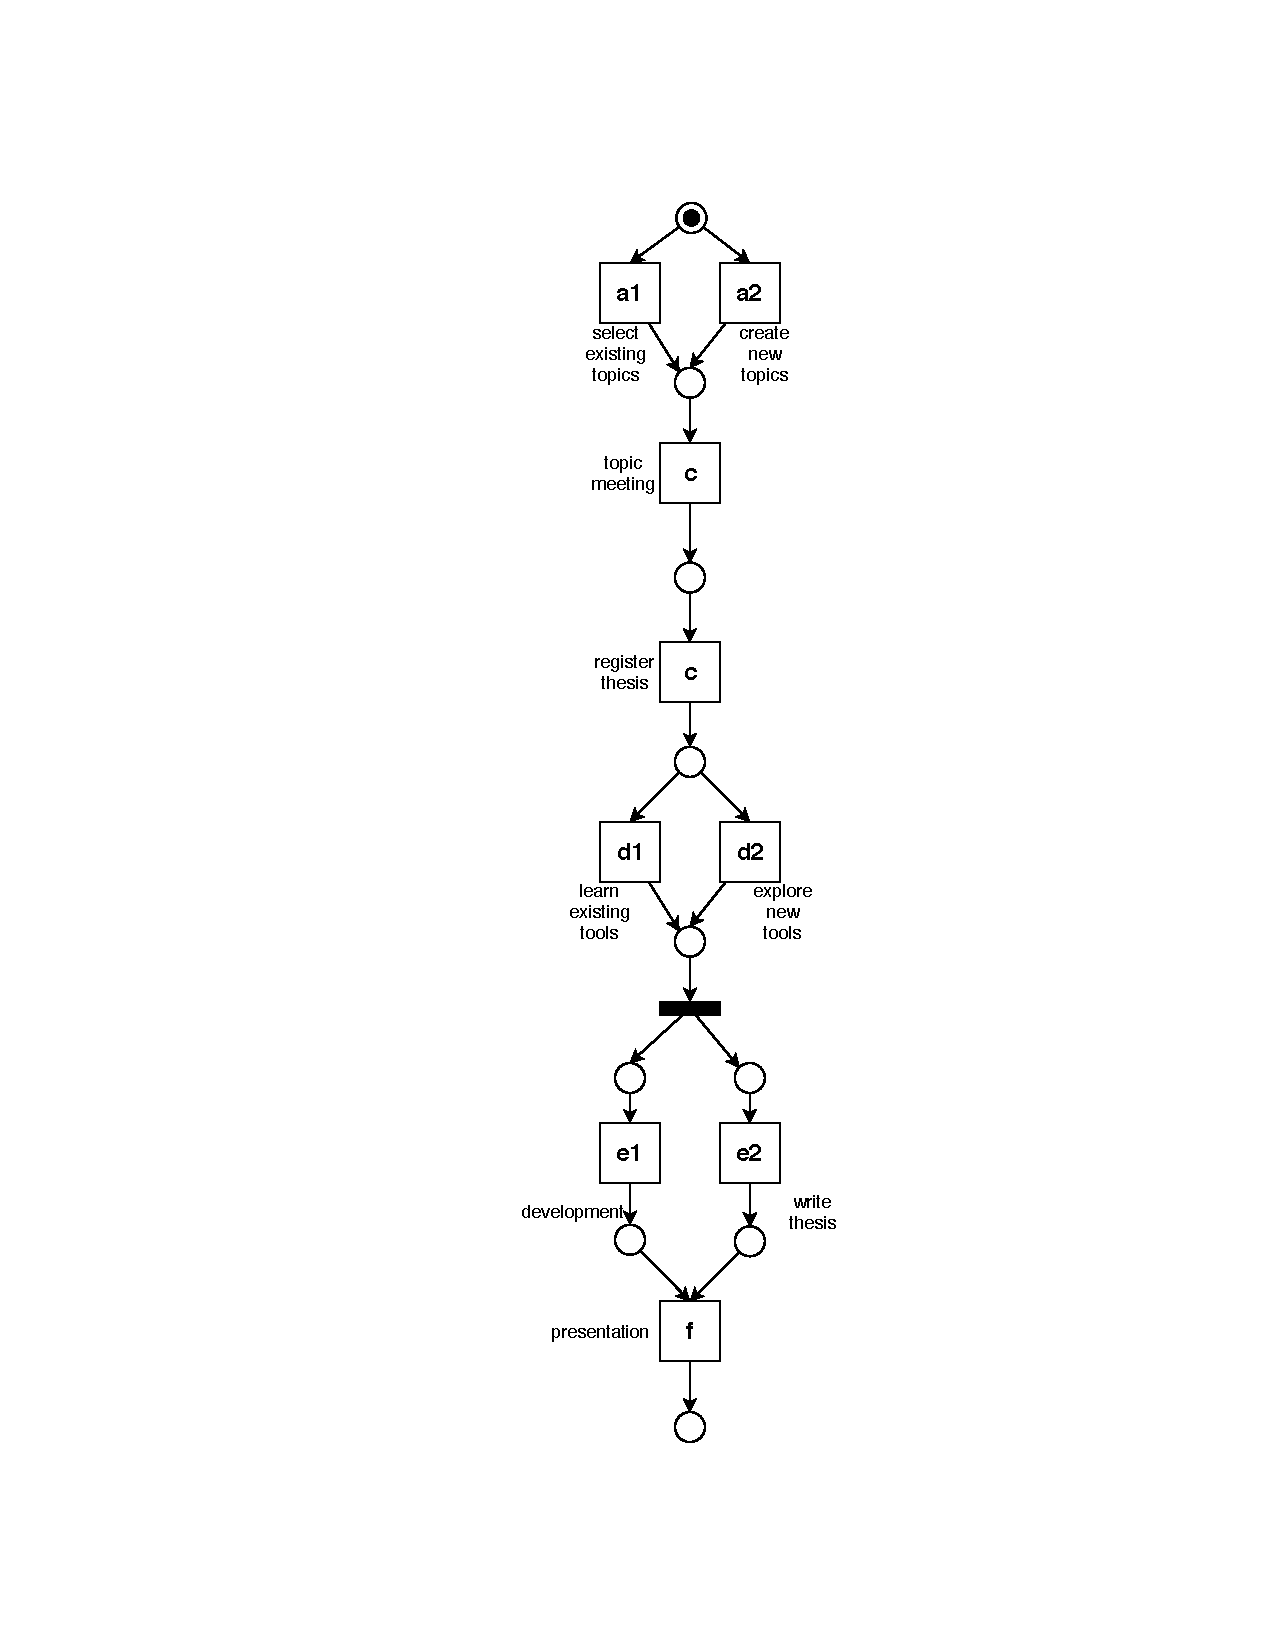
\includegraphics[clip, trim=8.5cm 3cm 7cm 3cm, width=0.4\textwidth, height=0.6\textheight]{figures/introduction/thesis-demo-final-original-model.pdf}
	\caption{The original master study process $M_0$.}
	\label{fig:demo-M0}
\end{wrapfigure} 

In the following sections, motivating examples are given to describe those limits of the current repair techniques in several situations. Then we propose research questions to overcome those limits and define our research scope. At the end, we give the outline for the whole thesis.
%% Motivation
\section{Motivating Examples}

For better understanding, examples are extracted from the common master thesis procedure to illustrate those situations. The process is described by the Petri net $M_0$ in Figure \ref{fig:demo-M0}. Activities are denoted as rectangle and connected by circles called places. The directed arcs in the Petri net indicate the execution order of activities. And the black dots in places of the model represents current execution states. In addition, those dots can be substituted by other symbols due to visualization tools, like numbers in places.

According to the model, a student can \textbf{select existing topics}  or \textbf{create new topics}. Those two activities are exclusive. The exclusive choice relation also exist in  \textbf{learn existing tools}  or \textbf{explore new tools}. Activities \textbf{development} and hold a \textbf{write thesis} are executed currently. Activity \textbf{presentation} is necessary to complete a master thesis project. For convenience, alphabets are used to represent the corresponding activities and annotated in the model later.

%% here we want to use one example to show the shortcomings of current repair methods.. How to organize them??? 
\subsection{Situation 1: \small{Add Subprocesses as Loops}} % add preparation to this model
One obvious shortcoming of repair techniques in \cite{fahland2015model} is that subprocesses for  deviations are created and added as loops, when the deviations start and end at the same place. If there is only one such subprocess, it is fixed as a sequence in the model with post procedure. Yet, the algorithm does not discover orders between different subprocesses at overlapping locations. Therefore, the subprocesses are kept in a loop form, which causes a lower precision of the repaired model. An example is given with respect to the master study. 

In some universities, before registering a master thesis, the activities \textbf{write proposal}, represented by \textbf{x1}  and \textbf{check course requirement}, represented by \textbf{x1}, are necessary for the whole procedure. We assume that traces with either of those activities are considered as positive.  

For convenience, the real process is recorded in the event log $L_1$ in the following way. Traces with the same activities order and the same label are summed together. The corresponding sum and label are listed above the whole sequence. For example, the first item in $L_1$ indicates that there are 50 traces which follow the order as ${<a1, b, \textbf{x1},c, d1, e1, e2, f>}$ and lead to positive performance outcomes.
\begin{align*}
		L_1:= \{ &  {<a1, b, \textbf{x1},c, d1, e1, e2, f>}^{50, pos}, \\   
		  &{<a1, b, \textbf{x2},c, d2, e1, e2, f>}^{50,pos},
		% & {<a,b,c1,d,\quad e, f1,g1,g2,h,i>}^{50, neg} 
		\}
		\end{align*}
When using rediscovery strategy with setting, the Inductive Miner for Infrequent and noise threshold with 20, a new  model $M_{1.2}$ based on the positive instances of $L_1$ is generated in Figure \ref{fig:demo_s1_IM}. \textbf{x1, x2} position with exclusive choices as implied by event log $L_1$. However, \textbf{a1} is kept in the new model and \textbf{a2} has been deleted, because no traces in $L_1$ includes \textbf{a2}.
		
		
Because the existing repair techniques  \cite{fahland2015model} don't consider the performance of traces in event log, all instances with negative labels are ignored to compute the deviations. $L_1$ has deviations of \textbf{x1, x2} at the same place without order. The corresponding subprocesses for them are added in the loop as shown in Figure \ref{fig:demo_s1_fahland}, which brings more behavior than expected into model.
\begin{figure}[htp]
	\centering
	\begin{subfigure}[b]{0.48\textwidth}
		\centering
		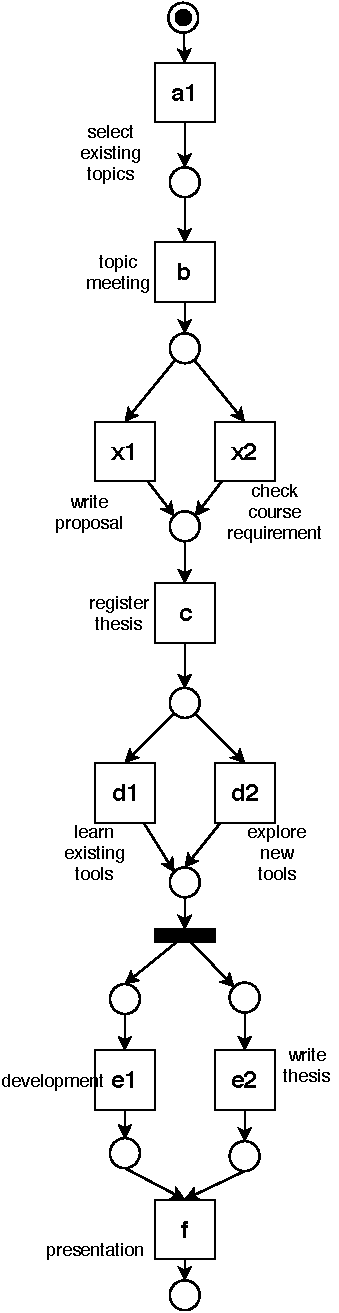
\includegraphics[ width=0.8\linewidth, height=0.8\textheight]{figures/introduction/thesis-demo-s1-IM.pdf}
		\caption{rediscovered model $M_{1.1}$ by IM}
		\label{fig:demo_s1_IM}
	\end{subfigure}
	\begin{subfigure}[b]{0.48\textwidth}
		\centering
		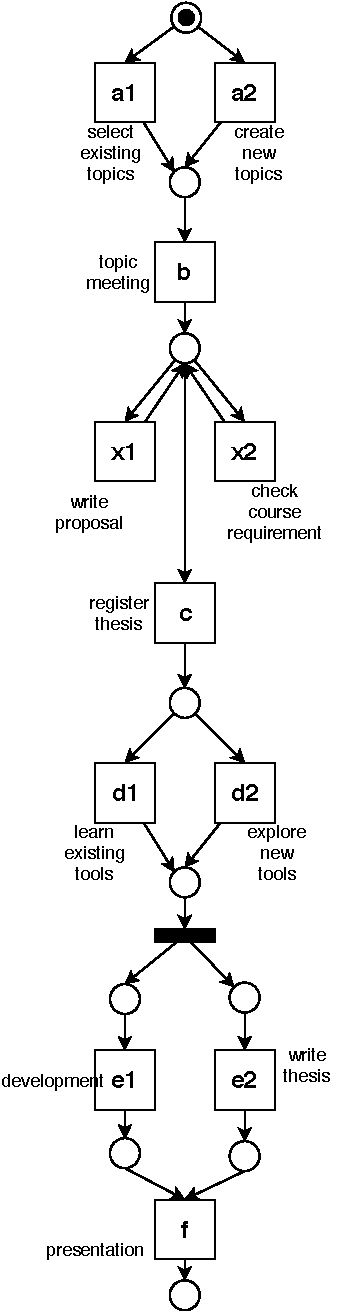
\includegraphics[width=0.8\linewidth, height=0.8\textheight]{figures/introduction/thesis-demo-s1-fahland.pdf}
		\caption{repaired model $M_{1.2}$ with techniques in \cite{fahland2015model}}
		\label{fig:demo_s1_fahland}
	\end{subfigure}%
	\caption[Motivating examples for situation 1]{Motivating examples for situation 1 where $M_{1.1}$ is rediscovered by Inductive Miner-Infrequent with threshold 0.2, and $M_{1.2}$ is repaired with techniques in \cite{fahland2015model} by adding subprocess in the form of loops.}
	\label{fig:demo_s1}
\end{figure}

The repair algorithm in  \cite{dees2017enhancing} builds upon  \cite{fahland2015model} and considers the performance of the event log. However, the repaired model is the same as the one in Figure \ref{fig:demo_s1_fahland}. The reasons are: (1) there is no deviation from negative factors. (2) positive deviations are used to add subprocesses in the same way as  \cite{fahland2015model}. 


Compared to the model $M_{1.1}$ and $M_{1.2}$ in Figure \ref{fig:demo_s1} where the two extra activities are shown in loop, or the main original structure has been changed, we expect the subprocesses with \textbf{x1, x2} can be added in sequence without affecting the main structure. In this way, the model has a higher precision of the repaired model, while keeping similar to original one. %the model in Figure \ref{fig:model_b2} is more expected with \textbf{x1, x2} in sequence and a higher precision.

\subsection{Situation 2: \small{Unable to Adapt Model with Fit Traces}}
% we should delete the prepare carefully and casually from the model. Only consider to add the data about the order change..what we expect is not 
This situation describes the existing problem in the current methods that fitting traces with negative performance outcomes cannot be used to repair a model. Given an actual event log $L_2$, The execution order of \textbf{development, write thesis} affects the performance outcomes. When \textbf{development} is executed before \textbf{write thesis}, more positive instances are given. In contrast, when \textbf{write thesis} is executed before \textbf{development}, more negative instances are caused. 
\begin{align*}
L_2:=\{ & { < a1, b, c, d2, \textbf{e1, e2}, f>}^{30, pos} , \\   
&{< a2, b, c, d1, \textbf{e1, e2}, f>}^{20, pos};   \\
&{< a2, b, c, d2, \textbf{e2, e1}, f>}^{10, pos}; 
& {< a1, b, c, d2, \textbf{e2, e1}, f>}^{20, neg} , \\
&{< a1, b, c, d1, \textbf{e2, e1}, f>}^{20, pos}; 
& {<a2, b, c, d1, \textbf{e1, e2}, f>}^{5, neg}  \}
\end{align*}
Compared to $M_0$, the event log $L_2$ contains no deviation. When we apply the techniques in  \cite{fahland2015model} and  \cite{dees2017enhancing} to repair the model, the model remains unchanged. Also, IM mines the same model as the original one. Apparently, the fact that those two methods can't incorporate the negative information in fitting traces causes this shortcoming. A model as $M_2$ is expected because it enforces the positive instances and avoids the negative instance. Unfortunately, the current methods don't allow us to obtain such results. 
\begin{figure}[htp]
	\centering
	\begin{subfigure}[b]{0.5\textwidth}
		\centering
		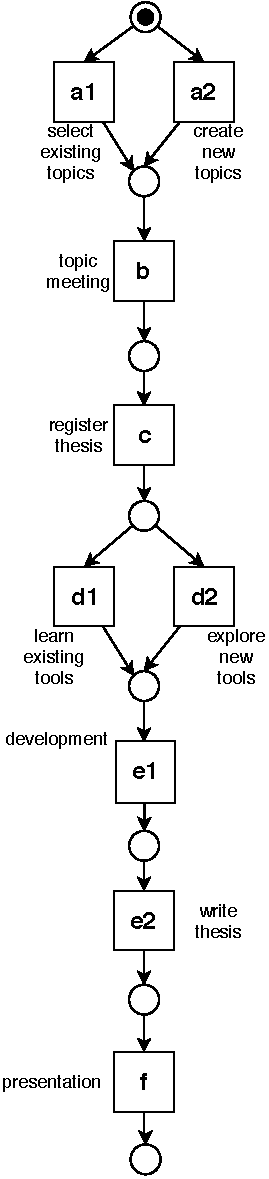
\includegraphics[ width=0.8\linewidth, height=0.8\textheight]{figures/introduction/thesis-demo-s2-expected.pdf}
		\caption{model $M_{2}$ with order change}
		\label{fig:demo_s2_order}
	\end{subfigure}%
	\begin{subfigure}[b]{0.5\textwidth}
		\centering
		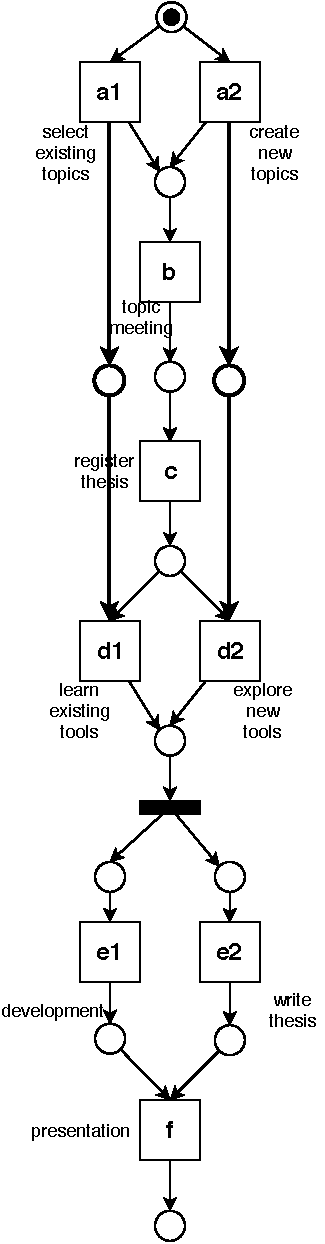
\includegraphics[width=0.8\linewidth, height=0.8\textheight]{figures/introduction/thesis-demo-s3-lt.pdf}
		\caption{model $M_{3}$ with long-term dependency}
		\label{fig:demo_s3_expected}
	\end{subfigure}
	\caption[Motivating examples for situation 2 and 3]{Motivating examples for situation 2 and 3. Current repair techniques keep the original models unchanged and can not output $M_{2}$ and $M_{3}$. $M_2$ with order changes of e1 and e2 is able to enforce positive and block negative instances. $M_{3}$ with long-term dependency leads to better precision.}
	\label{fig:model_demo_2_3}
\end{figure}
\subsection{Situation 3: \small{Disable to Detect Long-term Dependency}}
Another problem is that current methods are unable to detect the long-term dependency in the Petri net, which causes a lower precision. The long-term dependency describes the phenomenon that the execution of an activity decides the execution of activities that do not follow directly. Due to the long distance of this dependency, current methods cannot detect it and improve the precision by adding long-term dependency on the model. One example  on $M_0$ is used to demonstrate this problem.
 

Given the time consumption on the whole study as the KPI, if the total sum goes over one threshold, the trace is negative, else as positive. Since the activity \textbf{create new topics} usually demands new knowledge rather than \textbf{checking the existing tools}. If students choose to learn existing tools, it's possibly not useful and time-wasting. In the other case, if we select existing topics with existing background, it saves time when we directly learn the existing tools. According to this performance standard, we classified those event traces into positive and negative shown above.
%here we list one example to explain the long-term dependency, but we need to make them clear, might without the loop item..It means that we need to change the whole model..
An event log $L_3$ is given in the following. 
\begin{align*}
L_3:= \{ & { <\textbf{a1}, b, c, \textbf{d1}, e1, e2, f >}^{50, pos}, \\  
 &{<\textbf{a2}, b, c, \textbf{d2}, e1, e2, f >}^{50, pos} ; \\
& {<\textbf{a1}, b, c, \textbf{d2}, e1, e2, f >}^{50, neg}, \\
& {<\textbf{a2}, b, c, \textbf{d1}, e1, e2, f >}^{50, neg}  \}
\end{align*}

As observed, \textbf{\emph{c1}} decides \textbf{\emph{f1}} while \textbf{\emph{c2}} decides \textbf{\emph{f2}}. They have long-term dependencies.
However, there are no deviations of the model and event log $L_3$ according to the  algorithms in  \cite{fahland2015model} and  \cite{dees2017enhancing}. Also, the Inductive Miner can't detect long-term dependency. Therefore, the original model stays the same and negative instances can't be blocked.

Clearly, the use of negative information can bring significant benefits, e.g, enable a controlled generalization of a process model: the patterns to generalize should never include negative instances. This leads to the demand of improving current repair model techniques with incorporating negative instances. In the next section, the demand is analyzed and defined in a formal way.

\section{Research Scope And Questions }
After analyzing the current model repair methods, we limit our research scope as shown in Figure \ref{fig:scope}.  The inputs for our research are one existing process model M, an event log L . According to predefined KPIs, each trace in event log is classified into positive or negative. After applying repair techniques in the black box, the model should be improved to enforce the positive instances while disallowing negative instance, with condition that the generated model should be as similar to the original model as possible. 
\begin{figure}
	\centering
	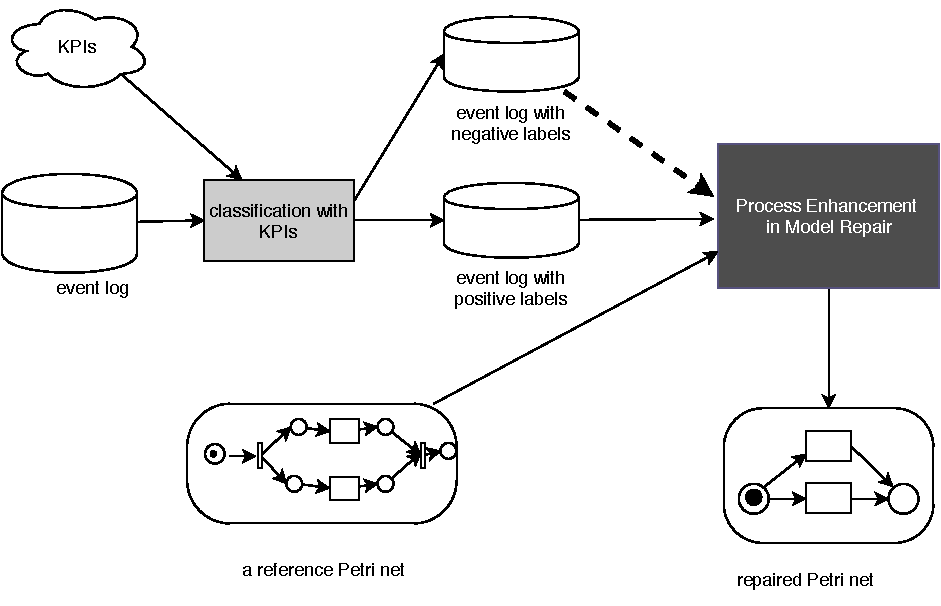
\includegraphics[width=\textwidth]{figures/introduction/P06-problem-scope.pdf}
	\caption[The reseach problem scope]{The scope shows the inputs for our problem is an event log and a process model in Petri net. According to certain KPIs, the event log is split into two event logs that are passed to repair the model. The output is also defined to be in the form of a Petri net. }
	\label{fig:scope}
\end{figure}

In this scope, we come up with several research questions listed in the following.
\begin{enumerate}[start=1,label={\bfseries{ RQ\arabic*:}}]
	%\itemsep0em
	\item How to overcome the shortcomings of current repair techniques in situations 1-3 above?
	\item How to balance the impact of the existing model, negative and positive instances together to repair model? 
	\item How to block negative instances from the model while enforcing the positive ones?
\end{enumerate}
  
In this thesis, we propose a solution for the black box. It analyzes process performance on trace level and balances the existing model, positive traces and negative traces on directly-follows relation, to incorporate all the factors on model generation. 

\section{Outline}
This thesis aims to answer the questions presented in section 1.2 in the remaining chapters and provides a solution for the black box. 
Chapter 2 introduces the related works. Chapter 3 recalls the basic notions on process mining and list the preliminaries to solve the problem. 
Chapter 4 firstly presents an original framework to incorporate negative information into model repair. Based on this framework, a concrete algorithm are proposed. 
In Chapter 5, screenshots of the implementation tools are shown to demonstrate the usage.  Chapter 6 answers the last question RQ3, by conducting a bundle of experiments. Later, results are analyzed and discussed. 
At last, we summarize our work in Chapter 7. 
%The next section answers the questions, how to balance all factors and block negative instances, Our algorithm analyzes process performance on trace level and balances the existing model, positive traces and negative traces on directly-follows relation, in order to incorporate all the factors on model generation. Long-term dependency is further detected on the intermediate model and added to block negative instances. What's more, the impact of the existing model, positive and negative instances are parameterized by weights, to allow more flexibility of the generated model.



%\end{document}